% !TEX TS-program = pdflatex
% !TEX encoding = UTF-8 Unicode

% This is a simple template for a LaTeX document using the "article" class.
% See "book", "report", "letter" for other types of document.

\documentclass[11pt]{scrartcl} % use larger type; default would be 10pt

\usepackage[utf8]{inputenc} % set input encoding (not needed with XeLaTeX)

%%% Examples of Article customizations
% These packages are optional, depending whether you want the features they provide.
% See the LaTeX Companion or other references for full information.

%%% PAGE DIMENSIONS
\usepackage{geometry} % to change the page dimensions
\geometry{a4paper} % or letterpaper (US) or a5paper or....
\geometry{margin=1in} % for example, change the margins to 2 inches all round
% \geometry{landscape} % set up the page for landscape
%   read geometry.pdf for detailed page layout information

\usepackage{graphicx} % support the \includegraphics command and options

% \usepackage[parfill]{parskip} % Activate to begin paragraphs with an empty line rather than an indent

\usepackage{indentfirst} %%%% CJ added this to indent paragraphs

%%% PACKAGES
\usepackage{booktabs} % for much better looking tables
\usepackage{array} % for better arrays (eg matrices) in maths
\usepackage{paralist} % very flexible & customisable lists (eg. enumerate/itemize, etc.)
\usepackage{verbatim} % adds environment for commenting out blocks of text & for better verbatim
\usepackage{subfig} % make it possible to include more than one captioned figure/table in a single float
% These packages are all incorporated in the memoir class to one degree or another...

%%% HEADERS & FOOTERS
\usepackage{fancyhdr} % This should be set AFTER setting up the page geometry
\pagestyle{fancy} % options: empty , plain , fancy
\renewcommand{\headrulewidth}{0pt} % customise the layout...
\lhead{}\chead{}\rhead{}
\lfoot{}\cfoot{\thepage}\rfoot{}

%%% SECTION TITLE APPEARANCE
\usepackage{sectsty}
\allsectionsfont{\sffamily\mdseries\upshape} % (See the fntguide.pdf for font help)
% (This matches ConTeXt defaults)

%%% ToC (table of contents) APPEARANCE
\usepackage[nottoc,notlof,notlot]{tocbibind} % Put the bibliography in the ToC
\usepackage[titles,subfigure]{tocloft} % Alter the style of the Table of Contents
\renewcommand{\cftsecfont}{\rmfamily\mdseries\upshape}
\renewcommand{\cftsecpagefont}{\rmfamily\mdseries\upshape} % No bold!

%%% END Article customizations

%%% The "real" document content comes below...

\title{AC290 EXTREME COMPUTING: FINAL REPORT}
\subtitle{Bleeding Edge}
\author{Gioia Dominedo, Christian Junge, Abhishek Malali and Isadora Nun}
%\date{} % Activate to display a given date or no date (if empty),
         % otherwise the current date is printed 

\begin{document}
\setcounter{secnumdepth}{0}
\maketitle
\setlength{\parindent}{5ex}

\section{Introduction}
%%%Discuss the problem at large, influence maximization problem, motivations and a quick summary of the work and outline

The Influence Maximization Problem examines the behavior of nodes of a graph influencing one another.  For this assignment, we are looking at a graph of nodes and the edges between them, and examining how the nodes within this graph activate one another.  The nodes represent individual Yelp reviewers within the United States, the edges represent the connections between these reviewers, and activating a node represents that reviewer being influenced by one of its connections.  The goal of this problem is to find the optimal set of starting nodes, that is, the set with the highest average number of nodes activated when the simulation is run repeatedly.  In this way, we can select an initial set of reviewers to target with advertising and incentives that will have the maximum influence that spreads throughout the network of Yelp reviewers.  \\

The influence process is simulated with the Independent Cascade, in which the starting nodes stochastically activate their connections throughout the graph.  The success of a particular set of starting nodes in activating other nodes within the graph is measured by the Influence function, which returns the average total number of nodes that are activated in many runs of the Independent Cascade.  \\
\\
\\
\\
For Christian To Fill In:\\
--------------------------Motivations---------------------------------------\\
--------------------------Quick Summary of Work-----------------------\\
--------------------------Outline--------------------------------------------\\
\\
%%%%%%%%%%   Motivations
%%%%%%%%%%   Quick summary of Work
%%%%%%%%%%   Outline

\section{Methods}
%%%   Method
%%%   Uncertainty on the influence function. F
%%%   Naive, Greedy and SA optimization methods. 
%%%   Parallelization. Methods of parallelization and sample code of spark

\begin{enumerate}[A)]

%\noindent
\item \textbf {Uncertainty on the Influence Function (F)}\\
\par
The influence function returns an expected value that has a certain amount of uncertainty due to the fact that it is estimated from a finite number of randomized simulations from within the large sample space of all possible outcomes.  While the standard error of the independent cascade function is endemic to a given set of starting nodes, regardless of the number of simulations, the standard error of the Influence function shrinks as the number of independent cascade simulations ($N$) increases.  Therefore, a larger number of simulations will yield a more precise estimate of the average influence for a given set.  This tightening of the standard error is proportional to $\frac{1}{N^{-1/2}}$, therefore, the uncertainty in the value of the Influence Function can only be reduced by increasing the number of simulations.  All optimization algorithms that use the Influence Function are impacted by its inherent uncertainty, so an unavoidable tradeoff exists between the uncertainty in Influence values used to find the optimal set and computation time. \\

%\noindent
\item \textbf {Optimization Methods} \\
\par

\begin{enumerate}[i.]
\item \textbf{Naive Method}\\
The Naive set of size $k$ contains the $k$ nodes with the highest number of edges.  The Naive Method is the fastest and simplest optimization method considered because it does not require running any simulations of the Independent Cascade.  This makes it suitable as a baseline for other methods.  
\\

\par
\item \textbf {Greedy Algorithm}\\
The Greedy Algorithm is a method for finding a starting set of size $k$ with a high number of activations without searching every possible set of starting nodes.  In its first iteration, it finds the single node that has the highest value of the influence function when run over over $N$ simulations.  In each subsequent iteration, it finds the next node which, when added to the starting set, returns the highest expected value of activated nodes when run over $N$ simulations.  In this way, additional starting nodes are incrementally added to the set which was previously determined to be the best set until the set contains $k$ starting nodes.\\ 

The limitation of the Greedy Algorithm is that by not considering every possible starting set, it may not find the true optimum.  Furthermore, it is impacted by uncertainty within the Influence Function. \\

\par
\item \textbf {Simulated Annealing}\\
Simulated Annealing is a process to stochastically find the optimal starting set of nodes.  This optimization process was developed for discrete search spaces where an exhaustive search would take a prohibitively long time.  In the case of the Maximum Influence Problem, testing all possible combinations of nodes would take a very long time, so simulated annealing is a sensible approach.  \\

The process works as follows: First, an initial set is randomly selected and the value of the influence function for $N$ simulations is calculated.  Then this starting set is perturbed by switching some of the starting nodes, and the expected value of this new set is calculated.  The next iteration of the algorithm will use either the newly perturbed set or the set from the previous iteration, and it will select which of these two sets to move forward with randomly with a probability that is related to the difference in "Energy" (in this case, how many more nodes one set activates versus the other set, denoted $\Delta E$) and the "temperature" ($T$) of that given point in the algorithm.  The temperature is a parameter that changes throughout the algorithm to adjust the probability of accepting the next starting set.  This probability of accepting a new set is given by the equation $P(X=j)=\exp({\frac{-\Delta E}{T}})$.  If the temperature is high, the algorithm is more likely to accept a new set even though it returned a lower value of the influence function.  Varying the temperature throughout the iterations of the algorithm allows it to consider sets of nodes that do not look promising at first glance, but may, with slight modification, yield better sets than those that were previously being considered.  \\

The advantages of the simulated annealing algorithm are that it can search a very large sample space without considering an extremely large set of possibilities, and that it does so in a strategic way by iterating upon promising tracks, but not constraining itself to one small subset of the sample space.  \\
\end{enumerate}

%\noindent
\item \textbf {Parallelization}\\
%%% Methods of parallelization and sample code of spark
\begin{enumerate}
\item \textbf{Greedy Algorithm} -
The Influence function lends itself very well to parallelization because individual runs of the Independent Cascade are relatively fast and do not depend on one another.  Also, with a cap on the number of cascade steps, each run of the Influence function should each take roughly the same amount of time.  Therefore, within both the Simulated Annealing algorithm and the Greedy algorithm, parallelizing the Independent Cascades within each run of the Influence function should lead to significant time improvements. The parallelization strategy for the Greedy algorithm will be to split the graph nodes over the partitions and independently run them over different cores since one computation does not affect the other.\\
\\
\\
-------------------------------------------------------------------------------\\
---------------------------Sample Spark Code-----------------------------\\
-------------------------------------------------------------------------------\\
------Also, I need to verify that these parallelization strategies are the ones that you used, and the wording of these sections can be improved----------------------\\
-------------------------------------------------------------------------------\\
\\
\item \textbf{Simulated Annealing} - 
This algorithm executes serially and the set of nodes on which the Simulated annealing operates in each iteration depend on the set of nodes from the previous iteration. Hence the parallelization cannot be carried out on the nodes as in the Greedy Algorithm. Instead, we can parallelize the Influence Function by parallelizing the $N$ runs of the Independent Cascade. Since each of the runs operates independently on a set of starting nodes, we can thereby reduce execution time of the Simulated Annealing Algorithm.  
\\
\\
------------------------------------------------------------------------------\\
--------------------------Sample Spark Code-----------------------------\\
------------------------------------------------------------------------------\\
\\


\end{enumerate}
\end{enumerate}


\section{Implementation and Results for NC mini and NC full}
%%% Choices of implementation and results (this should include all 3 algorithms) and understanding of the uncertainty (include all plots I have asked in class)   
\begin{enumerate}
\item \textbf{NC min}\\
We implemented the Naive, Greedy, and Simulated Annealing optimizations on the 240 node subset of the North Carolina graph to develop our code.  The results appear in Table 1:\\\
\\
--------------------------------------------------------------------------------------------------------\\
------------Influence------Run Time-------Optimal Nodes-----------------------------------------\\
---Naive----???------------???----------------???----------------------------------------------------\\
---Greedy--???------------???----------------???----------------------------------------------------\\
---SA-------???------------???----------------???----------------------------------------------------\\
---------------------------------------------------------------------------------------------------------\\
\\
\\
\begin{figure}[h!]
\centering
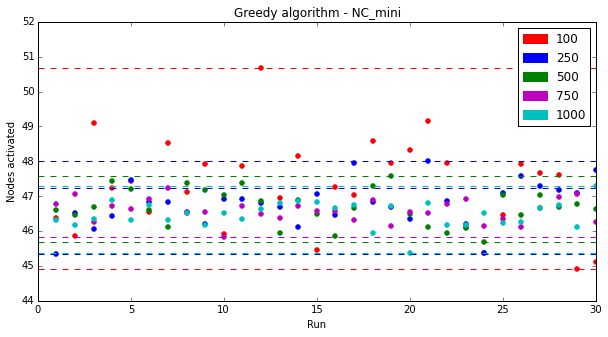
\includegraphics[width=15 cm]{greedy_min}
\label{fig_sim}
\caption{Plot demonstrating how minimum and maximum activations changes with respect to N}
\label{fig:GA}
\end{figure}

As can be seen in Figure 1, as the number of runs of the independent cascade within the greedy algorithm increases, the distance between the maximum and minimum activations decreases. The minimum bound also increases as expected with the increase in the number of runs for the greedy algorithm.  This means that uncertainty due to stochasticity in the influence function can be reduced by increasing the value of $N$.  There is a trade-off here, as increasing $N$ increases the amount of computation, and displays diminishing returns.  
\\
\\
---------------------------------------------------------------------------------------------------------\\
---------------------------------------------------------------------------------------------------------\\
----------------Plot showing how Simulated annealing goes up and down--------------------\\
----------Should have places where it flattens out, drops again, and comes back up before\\
-------------flattening out again to show that this was implemented properly----------------\\
-------Keep in mind that the Simulated Annealing Algorithm should store the absolute \\
max that it comes across (even though it will switch away from this as it heats and cools)---\\
------and should return the absolute max at the end------------------------------------------\\
------------------------------------------------------------------------------------------------------\\
------------------------------------------------------------------------------------------------------\\
\\
\begin{figure}
\centering
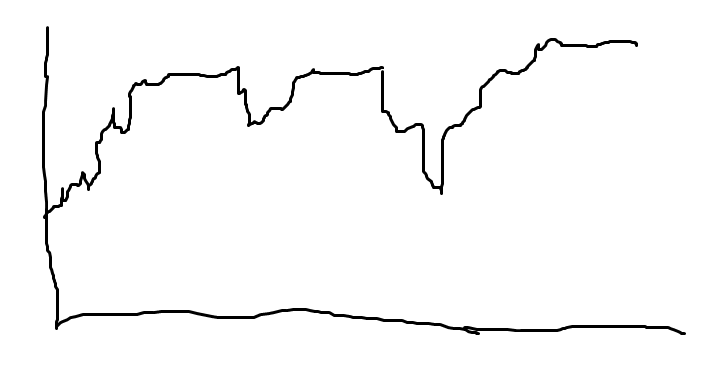
\includegraphics[width=10 cm]{SimAnFake}
\label{fig_sim}
\caption{Simulated Annealing}
\label{fig:LR}
\end{figure}

\item \textbf{NC full}\\
We implemented the same optimizations for the full 24,000 node graph of North Carolina reviewers, and the results appear in Table 2:\\
\\
----------------------------------------------------------------------------------------------------------\\
----------------------------------------------------------------------------------------------------------\\
------------Influence------Run Time-------Optimal Nodes-----------------------------------------\\
---Naive----???------------???----------------???----------------------------------------------------\\
---Greedy--???------------???----------------???----------------------------------------------------\\
---SA-------???------------???----------------???----------------------------------------------------\\
---------------------------------------------------------------------------------------------------------\\
----------------------------------------------------------------------------------------------------------\\
\\
\\
To reduce total compute time, the following restrictions were imposed on the Greedy Implementation for the full NC graph:\\
---------------------------------------------------------------------------------------------------------\\
----------------------------------------------------------------------------------------------------------\\
-------------------Cap depth?  Discussion of how the depth cap was selected, ideally an experiment where this was selected to shorten compute time without severely coming up short on the calculated influence------\\
----------------------------------------------------------------------------------------------------------\\
------------------Only consider nodes with connections, or with a min number of connections?----\\
----------------------------------------------------------------------------------------------------------\\
----------------Value of N, picked to be large enough to get good values of F, but small ----\\
-------enough to shorten compute time, discussion of how this N was selected systematically--\\
---------Refer to plot showing impact of N on uncertainty----------------------------------------\\
----------------------------------------------------------------------------------------------------------\\
\begin{figure}
\centering
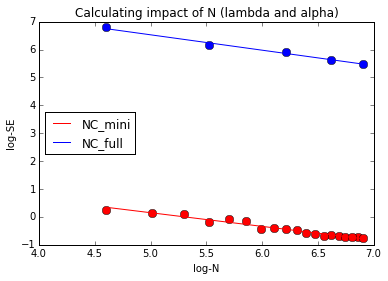
\includegraphics[width=10 cm]{LinearR}
%\label{fig_sim}
\caption{Estimating impact of N on uncertainty}
\label{fig:LR}
\end{figure}

\begin{figure}
\centering
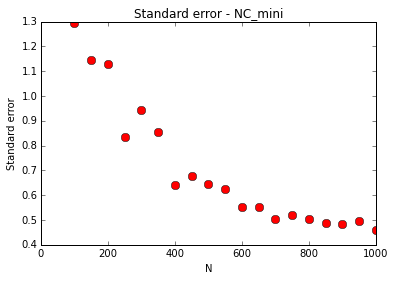
\includegraphics[width=10 cm]{StandardErrorVsN}
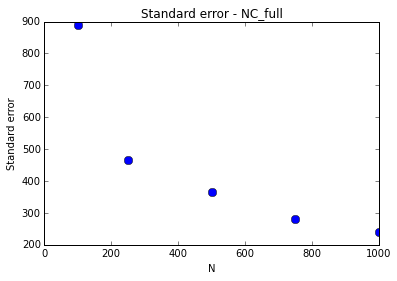
\includegraphics[width=10 cm]{StandardErrorVsNFull}
%\label{fig_sim}
\caption{Impact of N on uncertainty for greedy algorithm}
\label{fig:StandardError}
\end{figure}

---------------------------------------------------------------------------------------------------------\\
----------------------Plot of Simulated Annealing for NC Full------------------------------------\\
--------------------------------------------------------------------------------------------------------\\
\\
----------------------------------------------------------------------------------------------------------\\
------------Discussion of the parallelizations, with numbers and figures to support this-------\\
----------------------------------------------------------------------------------------------------------\\

Within the Simulated Annealing Algorithm, high levels of uncertainty in the value of the Influence Function for each set of starting nodes considered can cause the algorithm to fail to come to local maxima.  This is displayed conceptually in Figure 5 for the Traveling Salesman problem, where varying levels of uncertainty have been introduced into the distances between cities.  The ideal case is to be very certain of the distances so that the algorithm can converge properly on minimum distances.  Analogously in the Influence Maximization Problem, if the value of N is made too low to speed up computing time, Influence function values will be too noisy for the Simulated Annealing algorithm to converge on maximum influence values.  \\
\begin{figure}
\centering
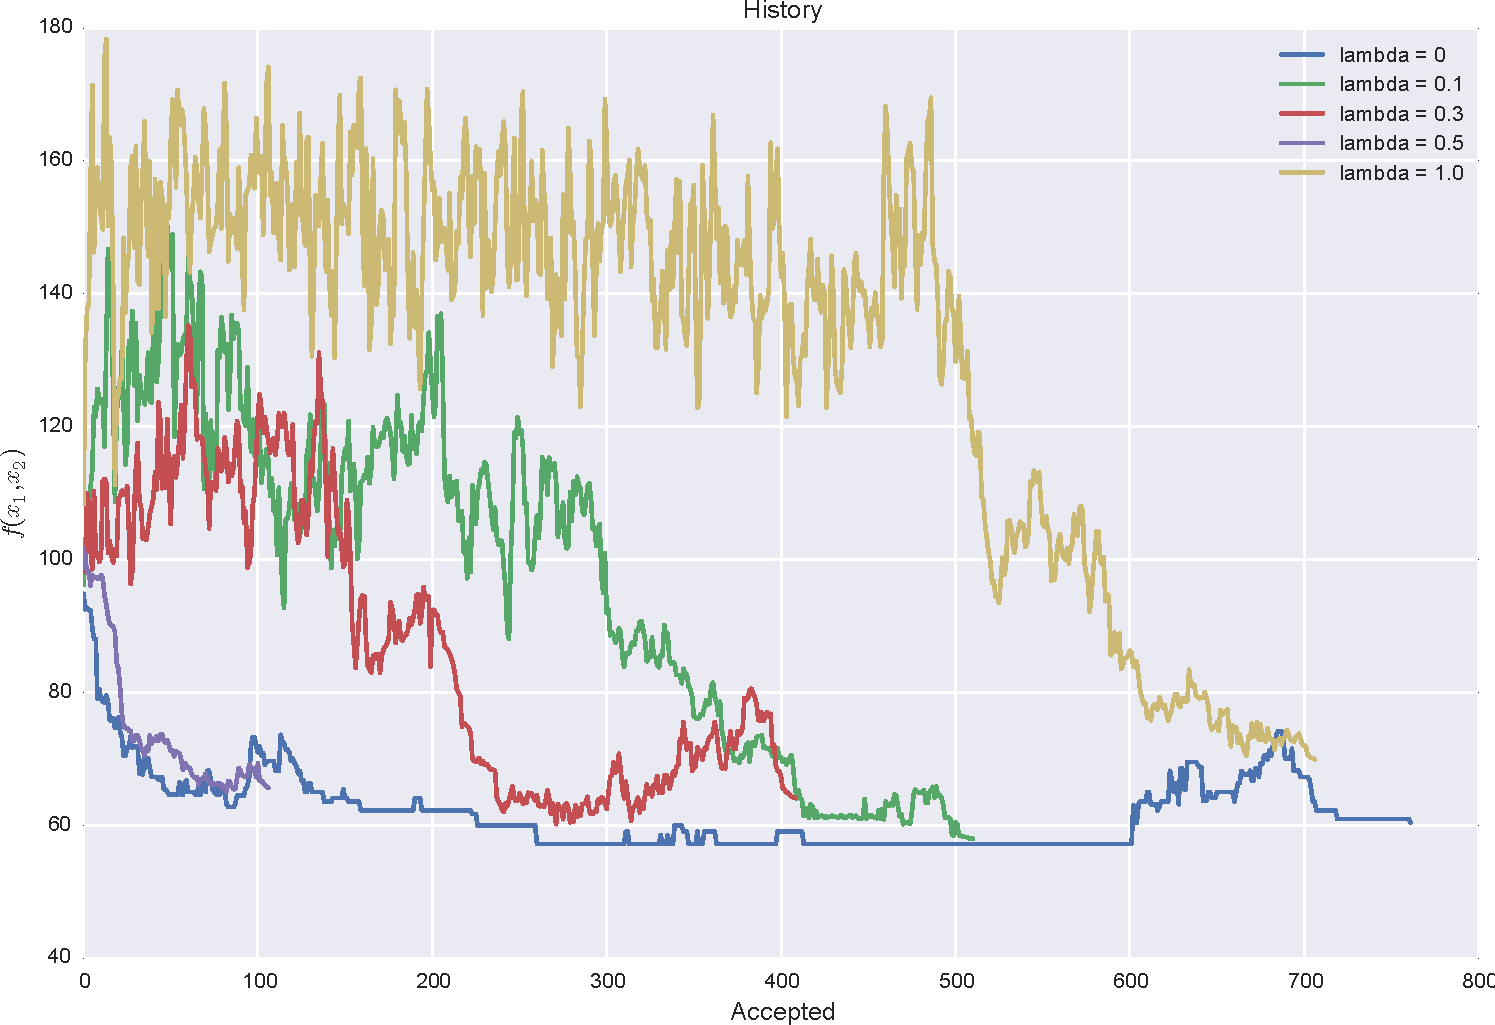
\includegraphics[width=10 cm]{lambda01}
%\label{fig_sim}
\caption{Simulated annealing with noise $= \lambda*random.uniform(0,1)$ for different values of $\lambda$}
\label{fig:SA}
\end{figure}

----------------------------------------------------------------------------------------------------------\\
----------------------------------------------------------------------------------------------------------\\
--If it is possible to make an analogous plot using different values of N for simulated annealing, even if it is just for NC mini, this would display this point better than the Traveling Salesman analog, and give more credibility to the value of N that we selected to use for Simulated Annealing\\
----------------------------------------------------------------------------------------------------------\\
----------------------------------------------------------------------------------------------------------\\

\end{enumerate}

\section{Scaling the algorithm to the US}
----------------------------------------------------------------------------------------------------------\\
----------------------------------------------------------------------------------------------------------\\
----------------------------------------------------------------------------------------------------------\\
----------------------------------------------------------------------------------------------------------\\
----------------------------------------------------------------------------------------------------------\\
 What strategy did you use to scale this problem?  Discussions can include:\\
 A) Balancing Noise vs Runtime tradeoff in selecting N (naturally, they should include a plot of standard deviation of influence vs N and runtime vs N)\\
 B) Reducing the depth of the cascade and its consequences\\
 C) Pruning methods - eliminating disconnected or low-out-degree nodes\\
 D) For SA: neighborhood selection - random vs direct neighboring node\\
----------------------------------------------------------------------------------------------------------\\
----------------------------------------------------------------------------------------------------------\\
----------------------------------------------------------------------------------------------------------\\
----------------------------------------------------------------------------------------------------------\\
\\
\\
\section{Conclusion}
A) Who are the top 3 influential reviewers?\\
B) Did your solution beat the Naive Method?\\
C) Future considerations: how could your algorithm be improved to solve this problem?\\
----------------------------------------------------------------------------------------------------------\\
----------------------------------------------------------------------------------------------------------\\
----------------------------------------------------------------------------------------------------------\\
----------------------------------------------------------------------------------------------------------\\
%
%









%\section{What is the problem?}
%
%\setlength{\parindent}{10ex}
%
%
%
%
%\section{What is Independent Cascading?}
%
%In the independent cascading approach, one or several nodes begin the simulation as activated.  The number of starting nodes is defined as $k$. In each iteration of the algorithm, each activated node has one chance to activate the nodes that it shares edges with.  The probability that an activated node ($v$) will activate a node adjacent to it ($w$) is given by the Beta function with the parameters $\alpha$ and $\beta$, where $\alpha$ is the number of reviews that reviewer $w$ has written after reviewer $v$ (within a time frame given by $\tau$), and $\beta$ is the total number of reviews that reviewer $w$ has written.  Within the algorithm, this is implemented by selecting a random number from the Beta distribution and a random number from the Uniform distribution, and if the number from the Uniform distribution is less than the number from the Beta distribution, the node is activated.  Each node gets only one chance to activate its non-activated neighbors, and the independent cascade algorithm terminates when there are no more possibilities to activate further nodes.  The algorithm returns the total number of nodes that have been activated in the simulation.  For the purpose of limiting total computation time, there is also an optional parameter $d$, or depth, that limits the number of cascade iterations that are permitted to run.  
%
%\section{What is the Influence Function?}
%
%The influence function is represented as follows:
%\begin{equation}
%f(S) = \frac{1}{N} \sum I(S)
%\end{equation}
%
%Where $N$ is the number of simulations, $f$ is the Influence function, $I$ is the independent cascade function, and $S$ is a given set of starting nodes.  The influence function tells the average number of nodes activated by a given set of starting nodes when the simulation is run N times, in other words, the expected value of the number of activated nodes.  In the Influence Maximization Problem, we would like to find the set S of starting nodes that yields the highest value of the Influence function.    
%
%
%\section{What is the Greedy Algorithm?}
%
%  
%

%
%\section{What is Simulated Annealing?}
%
%
%

%
%\section{Uncertainties in the Optimization}
%
%Uncertainty in the optimization results from stochastic approaches, which yield estimates with an unknown amount of error rather than definite values.  

%By fitting the data with a linear regression we obtain  $\frac{13.49}{N^{0.49}}$ for the mini-subset of the North Carolina graph and $\frac{10775}{N^{0.55}}$ for the full North Carolina graph. 
%	

%

%
%Also, as described above, there is uncertainty that either the Greedy Algorithm or the Simulated Annealing Algorithm will return the actual true optimal starting set with the maximum influence.  This is because neither approach considers every possible set of starting nodes, so either approach may fail to find the true optimal set.  \\
%
%
%	 

%	 
%\section{Distributed Computing}
%
%For the purposes of this problem, we considered the problem at three scales: a mini subset of all of the reviewers in North Carolina (240 nodes), the full set of all the reviewers in North Carolina (24,244 nodes), and the full set of all of the reviewers in the United States (350,620 nodes).  The purpose of breaking the set up in this way was to develop methods that could be run with a reasonable length of computing time, and then examine the issues related to scaling from a small subset to the entire set.  \\
%
%One of the issues with scaling the problem from the 240 node mini graph of North Carolina to the full set of 24,244 nodes is that individual runs of the iterated cascade could potentially run for many more iterations within a larger graph (particularly if many of the nodes in the graph were connected through chains and in isolated pockets, rather than being well connected within the whole set), so each cascade could take much longer to complete.  \\
%
%For this reason, we cap our cascade steps at 10.  The value of this cap $d$ also affects the scalability of number of starting nodes, which is described below.  Because of this, a smaller value of d will make the independent cascade run faster since the whole tree is not explored thanks to the depth cap $d$. In practice the effect of capping $d$ was\\
%%%%%%%%%%%%%%
% !!!!!!!!!!!!!!!!!!!!!!!!!!!!!!!!!!!!!!!!!!!!?\\
%%%%%%%%%%%%%%55
%
%Scaling $d$ was anticipated have much less of an impact on a small graph than it will on a large graph because in a smaller graph, the independent cascade is more likely to terminate before completing d cascades.  On a large graph, however, the independent cascade may run for many steps if the number of cascades is not capped.  Furthermore, the distribution of the number of cascades that may run is likely to be right-tailed, so even if the independent cascades are parallelized, one particularly long cascade may take much longer than its neighbors to run, thereby mitigating some of the benefits of parallelizing the Influence function.\\
%
%Scaling $N$ (the number of independent cascades run within calculations of the Influence function) should linearly increase the amount of computing time for the Influence function, because increasing the number of simulations does not increase the computing time of each.  As explained below, however, the Influence function lends itself well to parallelization, so increases in wall time can be minimized by parallelizing the Influence function.  As noted above, however, there are diminishing returns in the accuracy of the Influence function by scaling N, so some intermediate value of $N$ should give the optimal balance of low standard error and quick compute time.\\
%
%Scaling the number of starting nodes will have different impacts on the Simulated Annealing and Greedy Algorithms. In the Greedy algorithm, the first iteration considers the Influence of each of the $j$ nodes in the graph, and selects the node with the maximum influence.  The second iteration considers the Influence by adding each of $(j-1)$ remaining nodes, and so on to $(j-k)$.  For large graphs where $k$ (the number of starting nodes) is much smaller than $j$ (the total number of nodes in the graph), the difference between $j$ and $(j-k)$ is negligible, and so incrementing $k$ should lead to an essentially linear increase in computing time.  That is, adding another starting node should add an amount of computation that is not much less than the amount of computation for a single node.\\
%
%In the Simulated Annealing algorithm, changing the number of starting nodes will affect the amount of time for each independent cascade function, even though there is no increase in the time we take to make node swaps for the next iteration or to run the simulated annealing itself. Hence, for the Simulated annealing algorithm, the major bottle neck is the Independent cascade function. \\
%
%\section{Parallelization Strategies}
%

%\begin{figure}[h!]
%\centering
%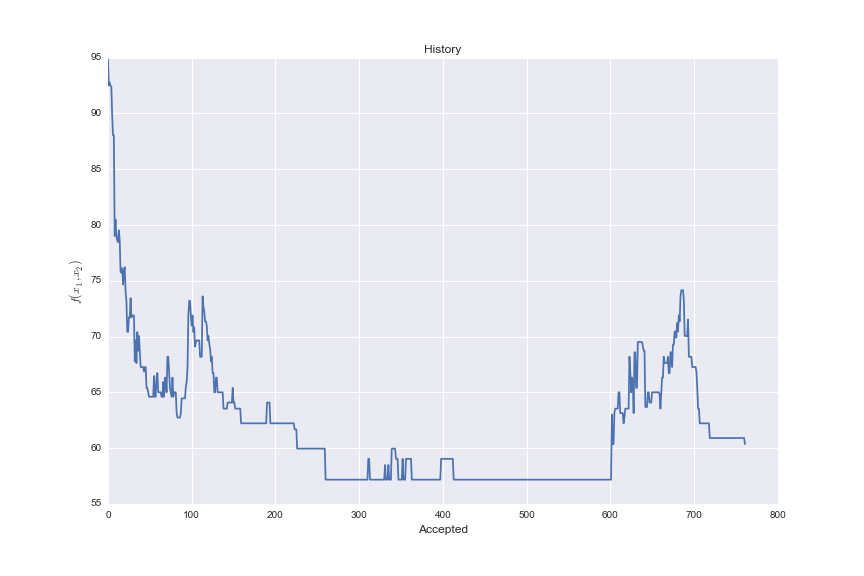
\includegraphics[width=10 cm]{SimAn}
%%\label{fig_sim}
%\caption{Simulated Annealing}
%\label{fig:SA}
%\end{figure}



\end{document}